\documentclass[preprint,12pt,aps,pra,showkeys,amsmath,amssymb,superscriptaddress,floatfix]{revtex4-2}
\usepackage[T1]{fontenc}
\usepackage[utf8]{inputenc}
\usepackage{amsmath,amssymb,amsthm,mathtools,mathrsfs}
\usepackage{microtype,booktabs,enumitem}
\usepackage{xcolor,tikz,etoolbox}
\usepackage[skins,breakable]{tcolorbox}
\usepackage{needspace}
% Keep diagram geometry independent of REVTeX preprint body spacing.
\AtBeginEnvironment{tikzpicture}{\linespread{1}\selectfont}
\usetikzlibrary{arrows.meta,positioning,calc,fit,decorations.pathreplacing}
\usepackage{graphicx}
\usepackage{hyperref}

\definecolor{MMBlue}{RGB}{0,82,155}
\definecolor{MMOrange}{RGB}{200,80,0}
\tikzset{
 mmnode/.style={draw=MMBlue,rounded corners=2pt,fill=MMBlue!4,align=left,execute at begin node={\raggedright},text width=5cm,font=\fontsize{10}{12}\selectfont,inner sep=6pt},
 mmimport/.style={mmnode,draw=black!65,fill=black!4},
 mmcandidate/.style={mmnode,draw=MMOrange,dashed,fill=MMOrange!5},
 mmrejected/.style={mmnode,draw=black,densely dotted,fill=black!8},
 mmproof/.style={->,thick,MMBlue},
 mmflow/.style={->,semithick,black!70},
 mmrepair/.style={->,dashed,thick,MMOrange},
 mmcandidatearrow/.style={->,dashed,semithick,MMOrange},
 mmnote/.style={font=\scriptsize,fill=white,inner sep=2pt,align=center}}

\usepackage[section]{placeins}
\setlength{\emergencystretch}{3em}
\setlist{itemsep=3pt,topsep=4pt}
\newtheorem{theorem}{Theorem}[section]
\newtheorem{proposition}[theorem]{Proposition}
\newtheorem{lemma}[theorem]{Lemma}
\newtheorem{corollary}[theorem]{Corollary}
\theoremstyle{definition}
\newtheorem{definition}[theorem]{Definition}
\newtheorem{example}[theorem]{Example}
\theoremstyle{remark}
\newtheorem{remark}[theorem]{Remark}
% Avoid isolated statement headings and single-line paragraph fragments.
\BeforeBeginEnvironment{theorem}{\Needspace{6\baselineskip}}
\BeforeBeginEnvironment{definition}{\Needspace{5\baselineskip}}
\BeforeBeginEnvironment{proposition}{\Needspace{5\baselineskip}}
\BeforeBeginEnvironment{lemma}{\Needspace{5\baselineskip}}
\BeforeBeginEnvironment{corollary}{\Needspace{5\baselineskip}}
\clubpenalty=5000
\widowpenalty=5000
\newcommand{\R}{\mathbb R}\newcommand{\Z}{\mathbb Z}\newcommand{\N}{\mathbb N}
\newcommand{\Pa}{\operatorname{Pa}}\newcommand{\Desc}{\operatorname{Desc}}
\newcommand{\cl}{\operatorname{cl}}\newcommand{\cost}{\operatorname{cost}}
\newcommand{\status}{\operatorname{status}}
% Faculty cards: a visual rail groups the five faculties within one agent.
% The rail has no arrowhead and does not represent a proof dependency.
\newcommand{\mmfacultybadge}[1]{%
 \node[circle,draw=MMBlue,line width=1pt,fill=white,
 minimum size=7mm,inner sep=0pt,font=\sffamily\small\bfseries,text=MMBlue]
 at ([xshift=15pt,yshift=-15pt]frame.north west) {#1};}
\newcommand{\mmfacultyrail}{%
 \draw[MMBlue!80,line width=1pt]
 ([xshift=15pt,yshift=2pt]frame.north west)--
 ([xshift=15pt,yshift=-2pt]frame.south west);}
\newtcolorbox{mmfacultybox}[2]{enhanced,breakable,
 colback=MMBlue!4,colframe=MMBlue!4,boxrule=0pt,arc=3pt,
 left=39pt,right=9pt,top=4pt,bottom=4pt,
 before skip=2pt,after skip=2pt,
 fontupper=\small\linespread{1.1}\selectfont,
 overlay unbroken={\mmfacultyrail\mmfacultybadge{#1}},
 overlay first={\mmfacultyrail\mmfacultybadge{#1}},
 overlay middle={\mmfacultyrail},overlay last={\mmfacultyrail}}
\newcommand{\mmfaculty}[3]{%
 \begin{mmfacultybox}{#1}{#2}
 {\sffamily\bfseries\color{MMBlue}#2}\par\smallskip #3
 \end{mmfacultybox}}
\newcommand{\agent}[9]{%
 \Needspace{8\baselineskip}
 \subsubsection{#1}
 \noindent\textbf{Object.} #2\par
 \noindent\textbf{Role.} #3\par\smallskip
 \mmfaculty{E}{Ego}{#4}
 \mmfaculty{M}{Memory}{#5}
 \mmfaculty{I}{Intellect}{#6}
 \mmfaculty{S}{Sense}{#7}
 \mmfaculty{A}{Action}{#8}
 \smallskip\noindent #9\par}

\usepackage{longtable,array,calc}
\providecommand{\tightlist}{\setlength{\itemsep}{2pt}\setlength{\parskip}{0pt}}
\makeatletter
\def\frontmatter@abstract@produce{\par\addvspace{\frontmatter@preabstractspace}%
\begingroup\prep@absbox\unvbox\absbox\post@absbox\endgroup
\addvspace{\frontmatter@postabstractspace}}
\makeatother
\newcommand{\field}[2]{\par\smallskip\noindent\textbf{#1.} #2\par}
\setlength{\emergencystretch}{5em}
\AtBeginEnvironment{verbatim}{\small\linespread{1.0}\selectfont}


\hypersetup{colorlinks=true,linkcolor=MMBlue,urlcolor=MMBlue,pdfauthor={Dibakar Sigdel}}

\begin{document}

\title{Liouville's Theorem and the Fundamental Theorem of Algebra\\[4pt]\large An End-to-End Meta-Math Walkthrough}

\author{Dibakar Sigdel}

\affiliation{Mindverse Computing LLC, Lynnwood, WA 98087, USA}

\date{October 2026}

\begin{abstract}

A complete authored walkthrough of liouville's theorem and the
fundamental theorem of algebra, with explicit mathematical contracts,
local verification gates, and reusable exports. The report presents the
target theorem, declared imports, a dependency graph, five-faculty node
contracts, a continuous proof, a worked example, and a hypothesis-repair
audit. It is an authored mathematical exposition, not a deployed-agent
transcript or a formal proof-assistant certificate.

\end{abstract}\maketitle\linespread{1.12}\selectfont

\noindent\textbf{CA-02 / Complex Analysis / Report v1}

\section{Target and import contract}

\begin{theorem}

Prove every bounded entire function is constant. Deduce that every
nonconstant complex polynomial has a complex root.

\end{theorem}

\subsection{Foundations and permitted imports}

Import CA-01 and differentiation under its contour integral on a disk:
\(f'(z_{0})=(2\pi i)^{-1}\oint f(z)/(z-z_{0})^{2}\) dz. The
differentiation is justified by a locally uniform denominator bound away
from the contour. Use connectedness of C and polynomial leading-term
estimates; do not import root existence. Also use the real mean value
theorem on a line segment and the extreme value theorem for continuous
real functions on compact disks.

\clearpage\section{Node interaction workflow}

\begin{center}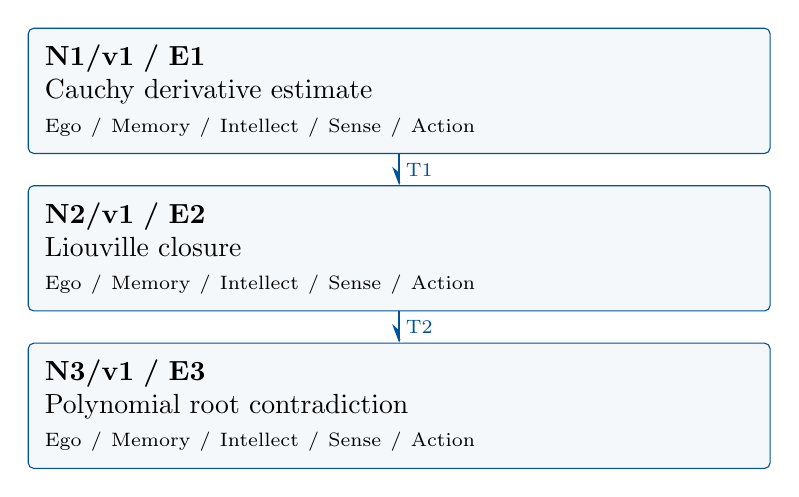
\begin{tikzpicture}[>=Stealth,x=1cm,y=1cm]

\node[mmnode,text width=9cm,minimum height=1.25cm] (N1) at (0,0.0) {\textbf{N1/v1 / E1}\\Cauchy derivative estimate\\{\scriptsize Ego / Memory / Intellect / Sense / Action}};

\node[mmnode,text width=9cm,minimum height=1.25cm] (N2) at (0,-2.0) {\textbf{N2/v1 / E2}\\Liouville closure\\{\scriptsize Ego / Memory / Intellect / Sense / Action}};

\node[mmnode,text width=9cm,minimum height=1.25cm] (N3) at (0,-4.0) {\textbf{N3/v1 / E3}\\Polynomial root contradiction\\{\scriptsize Ego / Memory / Intellect / Sense / Action}};

\draw[mmproof] (N1.south) -- node[mmnote,right] {T1} (N2.north);

\draw[mmproof] (N2.south) -- node[mmnote,right] {T2} (N3.north);

\end{tikzpicture}\end{center}

Each box is one mathematical agent containing all five faculties. Blue
arrows carry the versioned exports listed below. The layout gives a
reading order; only drawn arrows assert dependencies. Diagnostic repair
is separate from the proof DAG.

\subsection{Versioned evidence-transfer ledger}

\begingroup\small\linespread{1.05}\selectfont

\Needspace{5\baselineskip}\field{T1: N1/E1/v1 to N2}{Every derivative of order 1 vanishes.}

\field{Receiving activity}{N2: Liouville closure}

\field{Compatibility}{Use the same mathematical objects and hypotheses as the source export.
Receiving contract: Derivative zero everywhere; prior exports E1/v1}

\Needspace{5\baselineskip}\field{T2: N2/E2/v1 to N3}{Every bounded entire function is constant.}

\field{Receiving activity}{N3: Polynomial root contradiction}

\field{Compatibility}{Use the same mathematical objects and hypotheses as the source export.
Receiving contract: Nonconstant p of degree d with leading coefficient
\(a_d\ne 0\); prior exports E2/v1}

\endgroup

\clearpage\section{Agent roles and five-faculty activities}\begingroup\small\linespread{1.05}\selectfont\setlist{itemsep=1pt,topsep=2pt}

\subsection{N1/v1: Cauchy derivative estimate}

\field{Object and role}{Let a contour radius grow while the bound stays fixed.}

\field{Inputs}{Entire f with \(|f|\le M\) globally; foundational imports stated in §1}

\mmfaculty{E}{Ego}{Own E1/v1: Every derivative of order 1 vanishes.}

\mmfaculty{M}{Memory}{Retain Entire f with \(|f|\le M\) globally; foundational imports stated
in §1; keep their assumptions and versions attached.}

\mmfaculty{I}{Intellect}{Let a contour radius grow while the bound stays fixed.}

\mmfaculty{S}{Sense}{A bound depending on R cannot be sent to infinity this way.}

\mmfaculty{A}{Action}{Carry out the numbered deductions and publish E1/v1 together with its
hypotheses and proof location.}

\smallskip\noindent\textbf{Numbered mathematical activities}

\begin{enumerate}[label=N1.\arabic*,leftmargin=3.4em]

\item For any \(z_{0}\) and \(R>0\) the differentiated formula applies on the
disk about \(z_{0}\).

\item Its length \(2\pi R\) and denominator modulusR \(^{2}\) give
\(|f'(z_{0})|\le M/R\).

\item The same M holds for every radius since f is globally bounded.

\item Let \(R\to \infty\); \(f'(z_{0})=0\) for every \(z_{0}\).

\end{enumerate}

\field{Export E1/v1}{Every derivative of order 1 vanishes.}

\field{Acceptance gate}{A bound depending on R cannot be sent to infinity this way. Publish only
after checking every displayed deduction.}

\field{Targeted repair}{If the check fails, revise N1: A bound depending on R cannot be sent to
infinity this way. Recheck dependent nodes N2, N3.}

\clearpage

\subsection{N2/v1: Liouville closure}

\field{Object and role}{Use the connected domain to obtain one constant.}

\field{Inputs}{Derivative zero everywhere; prior exports E1/v1}

\mmfaculty{E}{Ego}{Own E2/v1: Every bounded entire function is constant.}

\mmfaculty{M}{Memory}{Retain Derivative zero everywhere; prior exports E1/v1; keep their
assumptions and versions attached.}

\mmfaculty{I}{Intellect}{Use the connected domain to obtain one constant.}

\mmfaculty{S}{Sense}{Zero derivative on a disconnected domain only gives componentwise
constancy.}

\mmfaculty{A}{Action}{Carry out the numbered deductions and publish E2/v1 together with its
hypotheses and proof location.}

\smallskip\noindent\textbf{Numbered mathematical activities}

\begin{enumerate}[label=N2.\arabic*,leftmargin=3.4em]

\item For any z,w, consider \(t\mapsto f(z+t(w-z))\) on{[}0,1{]}.

\item Its real parameter derivative is \(f'(z+t(w-z))(w-z)=0\); real and
imaginary parts are constant by the real mean value theorem.

\item Thus \(f(w)=f(z)\).

\item This proves Liouville's theorem on C.

\end{enumerate}

\field{Export E2/v1}{Every bounded entire function is constant.}

\field{Acceptance gate}{Zero derivative on a disconnected domain only gives componentwise
constancy. Publish only after checking every displayed deduction.}

\field{Targeted repair}{If the check fails, revise N2: Zero derivative on a disconnected domain
only gives componentwise constancy. Recheck dependent nodes N3.}

\clearpage

\subsection{N3/v1: Polynomial root contradiction}

\field{Object and role}{Apply Liouville to a hypothetical entire reciprocal.}

\field{Inputs}{Nonconstant p of degree d with leading coefficient \(a_d\ne 0\); prior
exports E2/v1}

\mmfaculty{E}{Ego}{Own E3/v1: Every nonconstant complex polynomial has a complex root.}

\mmfaculty{M}{Memory}{Retain Nonconstant p of degree d with leading coefficient \(a_d\ne 0\);
prior exports E2/v1; keep their assumptions and versions attached.}

\mmfaculty{I}{Intellect}{Apply Liouville to a hypothetical entire reciprocal.}

\mmfaculty{S}{Sense}{Bound the reciprocal on the compact interior as well as at infinity.}

\mmfaculty{A}{Action}{Carry out the numbered deductions and publish E3/v1 together with its
hypotheses and proof location.}

\smallskip\noindent\textbf{Numbered mathematical activities}

\begin{enumerate}[label=N3.\arabic*,leftmargin=3.4em]

\item Assume p has no zero.

\item Then 1/p is entire.

\item Choose R so for \(|z|\ge R\) the sum of lower-degree terms is at most
\(|a_d\Vert z|^d/2\).

\item Thus \(|p(z)|\ge |a_d\Vert z|^d/2\) and \(|1/p(z)|\le 2/(|a_d|R^d)\)
outside.

\item On the closed radius-R disk continuity and nonvanishing give a positive
minimum of\textbar p\textbar, hence a finite reciprocal bound.

\item Liouville makes 1/p constant, whereas it tends to 0 at infinity and is
nowhere zero, contradiction.

\item Therefore p has a root.

\end{enumerate}

\field{Export E3/v1}{Every nonconstant complex polynomial has a complex root.}

\field{Acceptance gate}{Bound the reciprocal on the compact interior as well as at infinity.
Publish only after checking every displayed deduction.}

\field{Targeted repair}{If the check fails, revise N3: Bound the reciprocal on the compact
interior as well as at infinity. Withhold this terminal result until its
gate passes.}

\endgroup\clearpage\section{Continuous mathematical proof}\label{sec:proof}

Read these steps in order as one proof; the diagram is optional.
Numbered activities identify the specific constructions and deductions
owned by each node.

\subsection{§4.N1 --- Cauchy derivative
estimate}\label{n1-cauchy-derivative-estimate}

\begin{enumerate}
\def\labelenumi{\arabic{enumi}.}
\item
  For any \(z_{0}\) and \(R>0\) the differentiated formula applies on
  the disk about \(z_{0}\).
\item
  Its length \(2\pi R\) and denominator modulusR \(^{2}\) give
  \(|f'(z_{0})|\le M/R\).
\item
  The same M holds for every radius since f is globally bounded.
\item
  Let \(R\to \infty\); \(f'(z_{0})=0\) for every \(z_{0}\).
\end{enumerate}

\subsection{§4.N2 --- Liouville closure}\label{n2-liouville-closure}

\begin{enumerate}
\def\labelenumi{\arabic{enumi}.}
\item
  For any z,w, consider \(t\mapsto f(z+t(w-z))\) on{[}0,1{]}.
\item
  Its real parameter derivative is \(f'(z+t(w-z))(w-z)=0\); real and
  imaginary parts are constant by the real mean value theorem.
\item
  Thus \(f(w)=f(z)\).
\item
  This proves Liouville's theorem on C.
\end{enumerate}

\subsection{§4.N3 --- Polynomial root
contradiction}\label{n3-polynomial-root-contradiction}

\begin{enumerate}
\def\labelenumi{\arabic{enumi}.}
\item
  Assume p has no zero.
\item
  Then 1/p is entire.
\item
  Choose R so for \(|z|\ge R\) the sum of lower-degree terms is at most
  \(|a_d\Vert z|^d/2\).
\item
  Thus \(|p(z)|\ge |a_d\Vert z|^d/2\) and \(|1/p(z)|\le 2/(|a_d|R^d)\)
  outside.
\item
  On the closed radius-R disk continuity and nonvanishing give a
  positive minimum of\textbar p\textbar, hence a finite reciprocal
  bound.
\item
  Liouville makes 1/p constant, whereas it tends to 0 at infinity and is
  nowhere zero, contradiction.
\item
  Therefore p has a root.
\end{enumerate}

\hfill$\square$

\section{Worked orchestration}

The entire function \(e^z\) is nonconstant and is unbounded along
positive real z, consistent with Liouville. For \(p=z^{2}+1\), the
root-existence conclusion holds and the explicit \(factors(z-i)(z+i)\)
illustrate it.

\subsection{Boundary and hypothesis audit}

The function1/z is bounded \(on\{|z|\ge 1\}\) but has a pole at 0, so it
is not a counterexample to Liouville. Sense identifies the missing
entire-domain condition; a bounded function on the unit disk can also be
nonconstant.

\section{Illustrative failure and repair}

The following is an authored diagnostic scenario. Changed assumptions
define a new contract; they do not retroactively prove the original
statement.

\subsection{Failure and correction}
This is an authored teaching trace, not a recorded agent run.

\begin{enumerate}
\def\labelenumi{\arabic{enumi}.}
\tightlist
\item
  \textbf{Ego \(\to\) Memory:} register the §1 theorem, imports, and
  requested exports before beginning the proof.
\item
  \textbf{Intellect \(\to\) Action:} choose the bridges in §3 and carry
  out the numbered activities in §4; transmit only established E-exports
  along the §2 DAG.
\item
  \textbf{Sense \(\to\) responsible node:} test the specific
  boundary/failure in §5 and the node's individual audit. A failing
  candidate is withheld; downstream nodes may not use it.
\item
  \textbf{Memory + Intellect:} identify whether the error is an omitted
  condition, an invalid inference, or an attempted extension beyond the
  theorem. Restore the exact contract or explicitly state a different
  one.
\item
  \textbf{Action:} redo the affected mathematical activity using the
  repaired condition or inference. Recheck consuming nodes, rather than
  feeding their conclusions back as premises.
\item
  \textbf{Ego:} publish only the supported export with its assumptions
  and proof location. A hypothetical revised export is v2; the written
  proof here is the v1 exposition, not a claim that this repair was
  executed.
\end{enumerate}

\subsection{Hypothesis boundary}
The function1/z is bounded \(on\{|z|\ge 1\}\) but has a pole at 0, so it
is not a counterexample to Liouville. Sense identifies the missing
entire-domain condition; a bounded function on the unit disk can also be
nonconstant.

\subsection{Version and recheck}
Treat any changed assumption as a new contract. Recheck the revised
export and all of its descendants. A backward diagnostic never
establishes an earlier theorem. This is an authored teaching trace, not
an execution log.

\par\medskip\begingroup\small\linespread{1.0}\selectfont\noindent\textbf{Provenance.} This authored proof is complete relative to its declared imports. Reuse
each export with its assumptions, proof, and version. The original
Markdown remains available for comparison.
\par\endgroup

\par\smallskip\begingroup\small\linespread{1.0}\selectfont\noindent\textbf{Further reading.} \begin{itemize}
\tightlist
\item
  \href{https://people.math.harvard.edu/~siu/math113/}{Harvard complex
  analysis: Cauchy formula, argument principle, and Riemann mapping
  lectures}.
\end{itemize}\par\endgroup

\end{document}
